\section{User Guide}
This section contains conceptual overviews of the code and clear examples for the prospective user. 

\subsection{Code Diagram}
The diagram in Fig. \ref{img:codeFlow} demonstrates the basic logic of the IMU module. There is additional code that deals with auxiliary functions.  An example of IMU use is given in test\_imu\_sensor.py in the imu\_sensor \_UnitTest folder. Application of each IMU function follows a simple, linear progression until realistic IMU outputs are achieved and sent out via the messaging system.

\begin{figure}[H]
	\centering 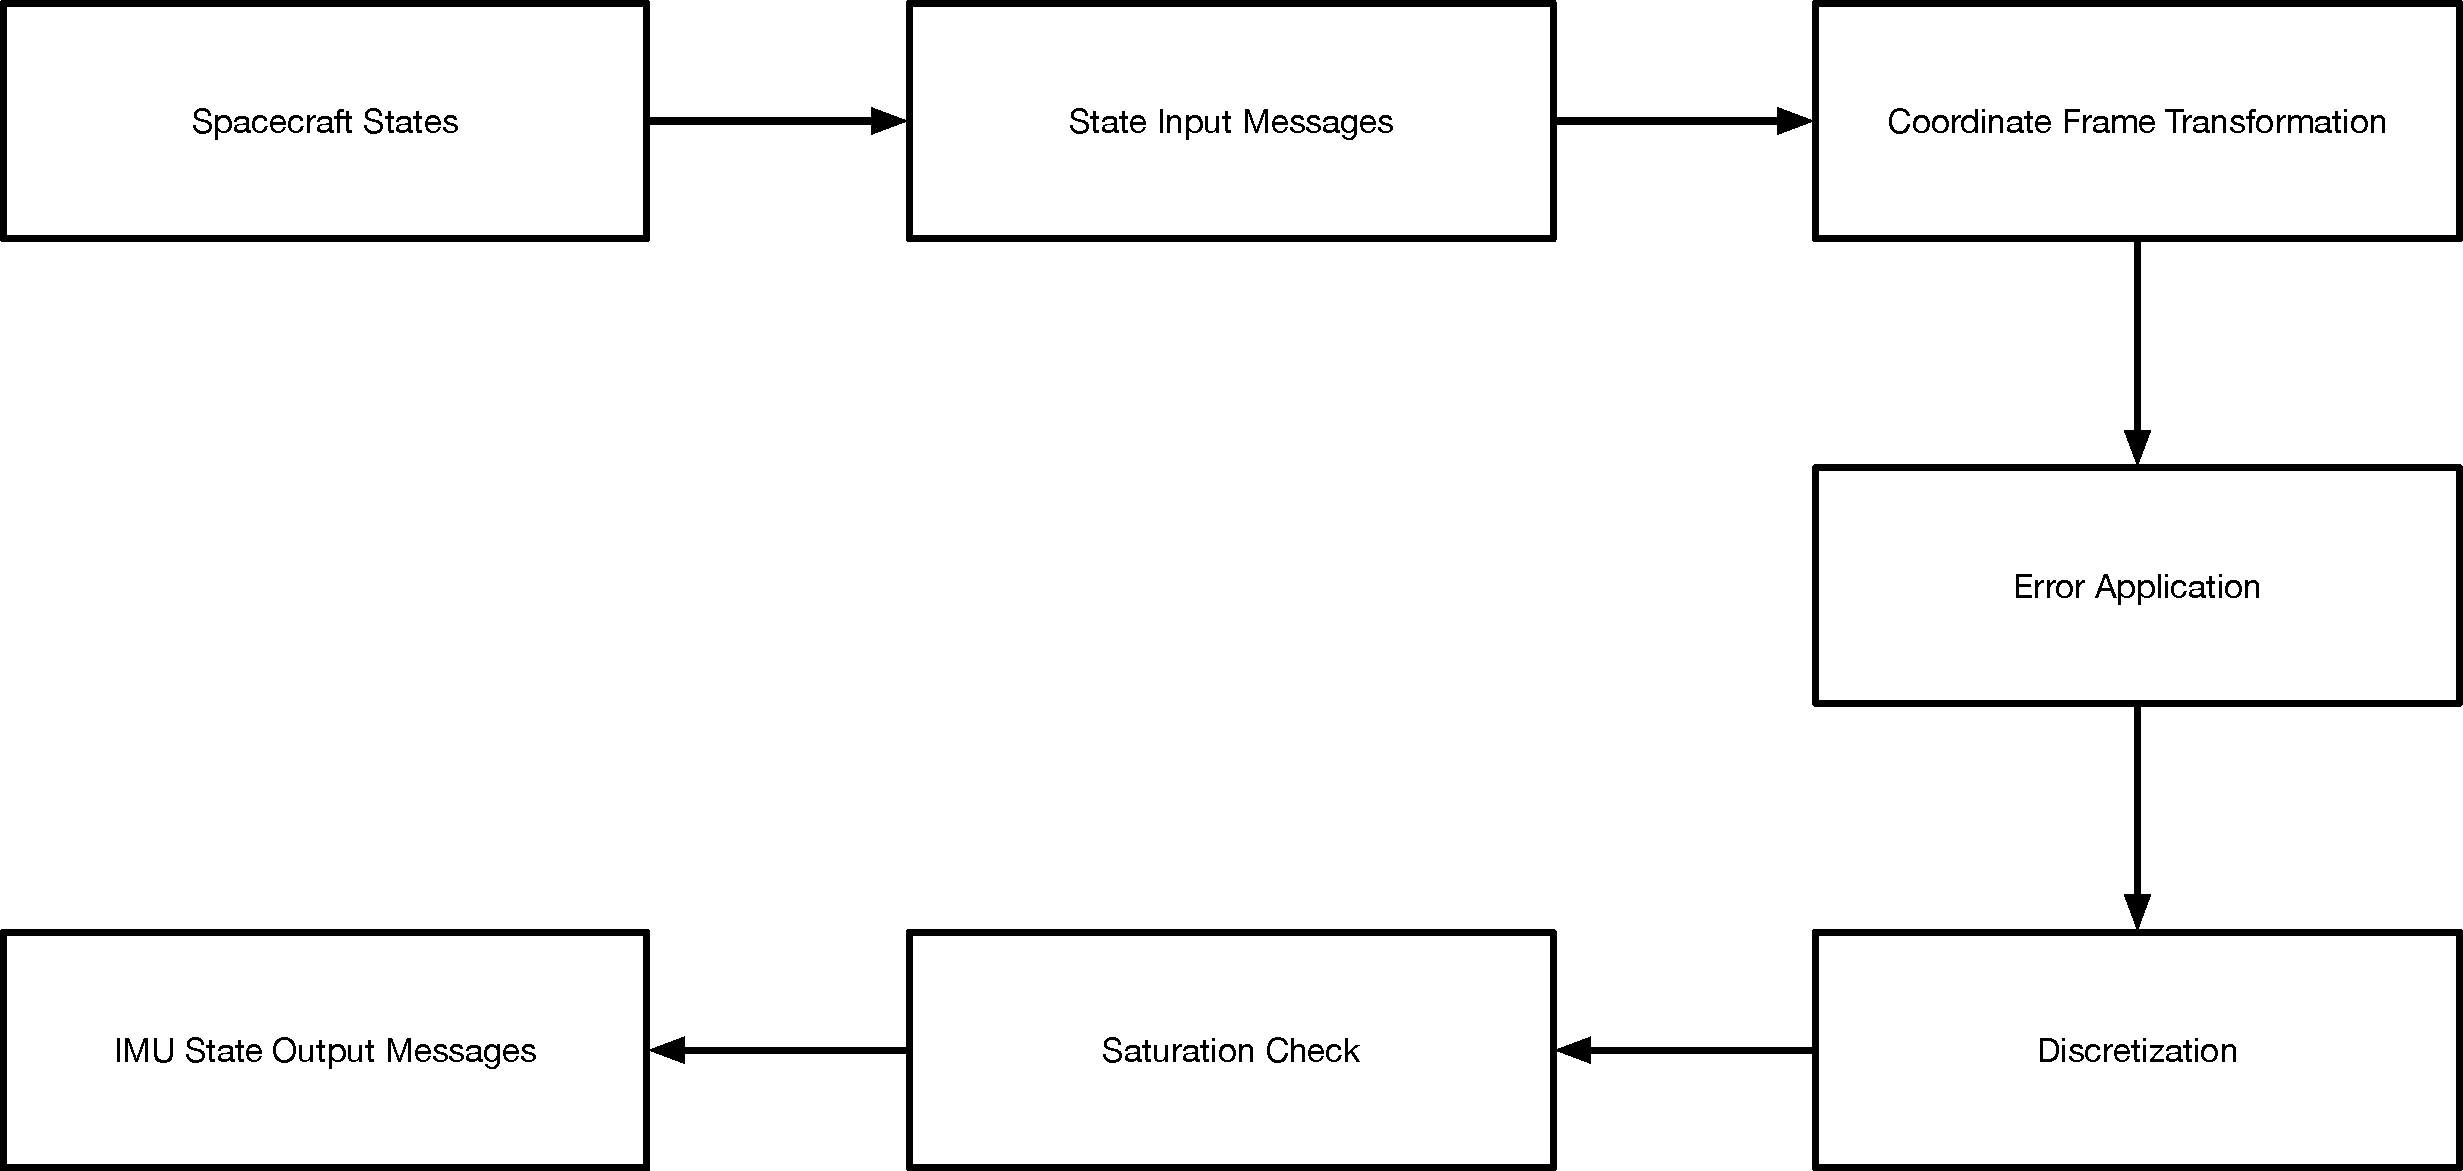
\includegraphics[height=0.4\textwidth, keepaspectratio]{Figures/codeFlow.pdf}
	\caption{A pseudo-code diagram demonstrating the flow of inputs and outputs in the IMU module.}
	\label{img:codeFlow}
\end{figure}

\subsection{Variable Definitions}
The variables in Table \ref{tabular:vars} are available for user input. Variables used by the module but not available to the user are not mentioned here. Variables with default settings do not necessarily need to be changed by the user, but may be.
\begin{table}[H]
	\caption{Definition and Explanation of Variables Used.}
	\label{tab:errortol}
	\centering \fontsize{10}{10}\selectfont
	\begin{tabular}{ | m{3cm}| m{3cm} | m{3cm} | m{6cm} |} % Column formatting, 
		\hline
		\textbf{Variable}   							& \textbf{LaTeX Equivalent} 	&		\textbf{Variable Type} & \textbf{Notes}			  \\ \hline
		InputStateMsg&N/A		   & string & Default setting: "inertial\_state\_output". This is the message from which the IMU receives spacecraft inertial data.\\ \hline
		OutputDataMsg & N/A & string & Default setting: "imu\_meas\_data". This message contains the information output by the IMU. \\ \hline
		SensorPos\_B & N/A & double [3] & [m] Required input - no default. This is the sensor position in the body frame relative to the body frame.\\ \hline
		roll, pitch, yaw & N/A  & double, double, double& Default setting: (0,0,0). To set non-zero initial angles between imu and spacecraft body, call setBodyToPlatformDCM(roll, pitch, yaw) \\ \hline
		dcm\_PB & N/A & double [3][3] & Default setting: Identity. Setting dcm\_PB is equivalent to calling setBodyToPlatformDCM(roll, pitch yaw) above. Use one method or the other. \\ \hline
		senRotBias & $\mathbf{e}_{\mathrm{bias}}$ & double [3] & [r/s] Default setting: zeros. This is the rotational sensor bias value for each axis. \\ \hline
		senTransBias & $\mathbf{e}_{\mathrm{bias}}$ & double [3] & [m/s2] Default setting: zeros. This is the translational sensor bias value for each axis \\ \hline
		senRotMax & $\mathbf{m}_{\mathrm{sat,max}}$& double & [r/s] Required input - no default. This is the gyro saturation value. \\ \hline
		senTransMax & $\mathbf{m}_{\mathrm{sat,max}}$ & double & [m/s2] Required input - no default. This is the accelerometer saturation value. \\ \hline
		PMatrixAccel & N/A yet & double [3][3] & Default: zeros. This is the covariance matrix used to perturb the state. \\ \hline
		PMatrixGyro & N/A yet & double [3][3] & Default: zeros. This is the covariance matrix used to perturb the state. \\ \hline
		walkBoundsGyro & N/A yet& double [3] & Default: zeros. This is the "3-sigma" errors to permit for gyro states \\ \hline
		walkBoundsAccel & N/A yet & double [3] & Default: zeros. This is the "3-sigma errors ot permit for acceleration states. \\ \hline
		accelLSB & (LSB) & double & Default: 0.0. This is the discretization value (least significant bit) for acceleration. Zero indicates no discretization. \\ \hline
		gyroLSB & (LSB)  & double & Default: 0.0. This is the discretization value (least significant bit) for acceleration. Zero indicates no discretization. \\ \hline
	\end{tabular}
	\label{tabular:vars}
\end{table}